\documentclass[english,man]{apa6}

\usepackage{amssymb,amsmath}
\usepackage{ifxetex,ifluatex}
\usepackage{fixltx2e} % provides \textsubscript
\ifnum 0\ifxetex 1\fi\ifluatex 1\fi=0 % if pdftex
  \usepackage[T1]{fontenc}
  \usepackage[utf8]{inputenc}
\else % if luatex or xelatex
  \ifxetex
    \usepackage{mathspec}
    \usepackage{xltxtra,xunicode}
  \else
    \usepackage{fontspec}
  \fi
  \defaultfontfeatures{Mapping=tex-text,Scale=MatchLowercase}
  \newcommand{\euro}{€}
\fi
% use upquote if available, for straight quotes in verbatim environments
\IfFileExists{upquote.sty}{\usepackage{upquote}}{}
% use microtype if available
\IfFileExists{microtype.sty}{\usepackage{microtype}}{}

% Table formatting
\usepackage{longtable, booktabs}
\usepackage{lscape}
% \usepackage[counterclockwise]{rotating}   % Landscape page setup for large tables
\usepackage{multirow}		% Table styling
\usepackage{tabularx}		% Control Column width
\usepackage[flushleft]{threeparttable}	% Allows for three part tables with a specified notes section
\usepackage{threeparttablex}            % Lets threeparttable work with longtable

% Create new environments so endfloat can handle them
% \newenvironment{ltable}
%   {\begin{landscape}\begin{center}\begin{threeparttable}}
%   {\end{threeparttable}\end{center}\end{landscape}}

\newenvironment{lltable}
  {\begin{landscape}\begin{center}\begin{ThreePartTable}}
  {\end{ThreePartTable}\end{center}\end{landscape}}

  \usepackage{ifthen} % Only add declarations when endfloat package is loaded
  \ifthenelse{\equal{\string man}{\string man}}{%
   \DeclareDelayedFloatFlavor{ThreePartTable}{table} % Make endfloat play with longtable
   % \DeclareDelayedFloatFlavor{ltable}{table} % Make endfloat play with lscape
   \DeclareDelayedFloatFlavor{lltable}{table} % Make endfloat play with lscape & longtable
  }{}%



% The following enables adjusting longtable caption width to table width
% Solution found at http://golatex.de/longtable-mit-caption-so-breit-wie-die-tabelle-t15767.html
\makeatletter
\newcommand\LastLTentrywidth{1em}
\newlength\longtablewidth
\setlength{\longtablewidth}{1in}
\newcommand\getlongtablewidth{%
 \begingroup
  \ifcsname LT@\roman{LT@tables}\endcsname
  \global\longtablewidth=0pt
  \renewcommand\LT@entry[2]{\global\advance\longtablewidth by ##2\relax\gdef\LastLTentrywidth{##2}}%
  \@nameuse{LT@\roman{LT@tables}}%
  \fi
\endgroup}


\ifxetex
  \usepackage[setpagesize=false, % page size defined by xetex
              unicode=false, % unicode breaks when used with xetex
              xetex]{hyperref}
\else
  \usepackage[unicode=true]{hyperref}
\fi
\hypersetup{breaklinks=true,
            pdfauthor={},
            pdftitle={Handling missing data in smartphone location logs},
            colorlinks=true,
            citecolor=blue,
            urlcolor=blue,
            linkcolor=black,
            pdfborder={0 0 0}}
\urlstyle{same}  % don't use monospace font for urls

\setlength{\parindent}{0pt}
%\setlength{\parskip}{0pt plus 0pt minus 0pt}

\setlength{\emergencystretch}{3em}  % prevent overfull lines

\ifxetex
  \usepackage{polyglossia}
  \setmainlanguage{}
\else
  \usepackage[english]{babel}
\fi

% Manuscript styling
\captionsetup{font=singlespacing,justification=justified}
\usepackage{csquotes}
\usepackage{upgreek}

 % Line numbering
  \usepackage{lineno}
  \linenumbers


\usepackage{tikz} % Variable definition to generate author note

% fix for \tightlist problem in pandoc 1.14
\providecommand{\tightlist}{%
  \setlength{\itemsep}{0pt}\setlength{\parskip}{0pt}}

% Essential manuscript parts
  \title{Handling missing data in smartphone location logs}

  \shorttitle{Missing Data in Smartphone Location Logs}


  \author{Boaz Sobrado\textsuperscript{1}}

  % \def\affdep{{""}}%
  % \def\affcity{{""}}%

  \affiliation{
    \vspace{0.5cm}
          \textsuperscript{1} Utrecht University  }

  \authornote{
    Department of Methodology \& Statistics
    
    Submitted as a research report conforming to APA manuscript guidelines
    (6th edition).
    
    Correspondence concerning this article should be addressed to Boaz
    Sobrado, . E-mail:
    \href{mailto:boaz@boazsobrado.com}{\nolinkurl{boaz@boazsobrado.com}}
  }


  \abstract{Using objective location data to infer the mobility measures of
individuals is highly desirable, but methodologically difficult. Using
commercially gathered location logs from smartphones holds great
promise, as they have already been gathered, often span years and can be
associated to individuals. However, due to technical constraints this
data is more sparse and inaccurate than that produced by specialised
equipment. In this paper we present a model which leverages the
periodicity of human mobility in order to impute missing data values.
Moreover, we will assess the performance of the model relative to
currently used methods, such as linear interpolation.}
  \keywords{Missing Data, Measurement Bias, GPS, Human Mobility \\

    \indent Word count: 2297
  }





\usepackage{amsthm}
\newtheorem{theorem}{Theorem}[section]
\newtheorem{lemma}{Lemma}[section]
\theoremstyle{definition}
\newtheorem{definition}{Definition}[section]
\newtheorem{corollary}{Corollary}[section]
\newtheorem{proposition}{Proposition}[section]
\theoremstyle{definition}
\newtheorem{example}{Example}[section]
\theoremstyle{definition}
\newtheorem{exercise}{Exercise}[section]
\theoremstyle{remark}
\newtheorem*{remark}{Remark}
\newtheorem*{solution}{Solution}
\begin{document}

\maketitle

\setcounter{secnumdepth}{0}



How people move about in their environment affects a wide range of
outcomes, such as health, income and social capital (Goodchild \&
Janelle, 2010). A better understanding of mobility could lead to better
health and urban-planning policies. Yet a large part of studies on human
mobility are conducted with pen-and-paper travel diaries, despite well
known methodological flaws. The high cost and burden to respondents
limits the span of data collection. Short trips are frequently
under-reported (Wolf, Oliveira, \& Thompson, 2003) . The self-reported
duration of commutes is often underestimated (Delclòs-Alió, Marquet, \&
Miralles-Guasch, 2017).

These obstacles can be overcome by using objective data on human
mobility. Such data can now be obtained using the Global Positioning
System (GPS). GPS uses the distance between a device and several
satellites to determine location. GPS measurements can be used to infer
a vast range of socioeconomic and behavioural measures, including where
the individual lives, how much time he or she spends at home and where
(and how) they travel.

Within behavioural sciences, researchers have used GPS data to
investigate wideranging topics. For example, Zenk, Schulz, and
Odoms-Young (2009) investigate the effects of the food environment on
eating patterns. G. M. Harari et al. (2016) look at the movement
correlates of personality, finding that extrovers individuals spend less
time at home than introverts. Wang, Harari, Hao, Zhou, and Campbell
(2015) looks at how academic performance is affected by movement
patterns. Palmius et al. (2017) use mobility patterns to predict bipolar
depression.

In most studies participants receive a specialised GPS devices to track
their movement. We call resulting logs \emph{specialised logs}. Barnett
and Onnela (2016) point out several methodological issues with these
studies. Like studies using pen-and-paper travel diaries, collecting
specialised logs is costly and places a high burden on participants.
Besides, introducing a new device to the participant's life may bias
their behaviour. Due to these drawbacks specialised logs usually span a
short amount of time. Barnett and Onnela (2016) advocate installing a
custom-made tracking app on user's phones (\emph{custom logs}). Another
solution is to take advantage of existing smartphone location logs
(\emph{secondary logs}) . For instance, Google Location History contains
information on millions of users (Location History, 2017). Often,
secondary logs span several years. By law, secondary logs are accessible
to users for free (Commission, 2017). Yet, secondary logs also present
methodological challenges. They were created for non-academic purposes
under engineering constraints (detailed subsequently). These constraints
mean that sensors do not track users continuously, meaning that the
resulting logs can be sparse and inaccurate. Hence, two important
challenges are dealing with measurement noise and missing data.

Missing data is a pervasive issue as it can arise due to several
reasons. Technical reasons include signal loss, battery failure and
device failure. Behavioural reasons include leaving the phone at home or
switching the device off. As a result, secondary logs often contain wide
temporal gaps with no measurements. For instance, several research
groups studying mental health report missing data rates between 30\% to
50\% (Grünerbl et al., 2015; Palmius et al., 2017; Saeb et al., 2015).
Other researchers report similar trends in different fields (e.g. G. M.
Harari et al., 2016; Jankowska, Schipperijn, \& Kerr, 2015).

There is no golden standard for dealing with missing data in GPS logs
(Barnett \& Onnela, 2016). Importantly, spatiotemporal measurements are
often correlated in time and space. This means that common methods, such
as mean imputation, are unsuitable. For example, imagine an individual
who splits almost all her time between work and home. Suppose she spends
a small amount of time commuting between the two along a circular path.
Using mean imputation to estimate her missing coordinates, we impute her
to be at the midpoint between home and work. She has never and will
never be there! Worryingly, there is little transparency on how
researchers deal with missing data (Jankowska et al., 2015).

The accuracy of smartphone location measurements is substantially lower
than that of professional GPS trackers. Android phones collect location
information through a variety of methods. Other than GPS measurements,
Androids use less-accurate heuristics such as WiFi access points and
cellphone triangulation. Different methods are used because of
computational and battery constraints. GPS is the most energy consuming
sensor on most smartphones (M. Y. Chen et al., 2006; LaMarca et al.,
2005). In professional GPS trackers less than 80\% of measurements fall
within 10 meters of the true location. GPS measures are most inaccurate
in dense urban locations and indoors (S. Duncan et al., 2013;
Schipperijn et al., 2014). Unfortunately for researchers, this is where
people in the developed world spend most of their time.

Noisy data can lead to inaccurate conclusions if it is not accounted
for. Suppose we wish to calculate an individual's movement in a day. A
simple approach would be to calculate the sum of the distance between
each measurement. But if there is noise, the coordinates will vary even
though the individual is not moving. If the measurements are frequent
and noisy, we will calculate a lot of movement, even if the individual
did not move at all! This issue is also visualised in Figure
\ref{fig:accuracyPlot}. The problem is further complicated because
missing data and noisy measurements are related. Methods used by
researchers to reduce noise, such as throwing out inaccurate
measurements (e.g. Palmius et al., 2017), can exacerbate the severity of
the missing data problem.

In this paper we will explore in detail the problem of missing data and
measurement error in secondary location logs. Moreover, we will compare
methods used to deal with these problems.

\subsection{A concrete example}\label{a-concrete-example}

There is little literature on dealing with missing data in custom or
secondary logs. Thus it is worth illustrating the typical
characteristics using an example data set. The example data set comes
from the Google Location History of a single individual. It spans from
January 2013 to January 2017 and contains 814 941 measurements. The data
set contains a multitude of variables, including inferred activity and
velocity. We will focus on measurements of latitude, longitude, accuracy
(defined below). All measurements are paired with a timestamp.

\subsubsection{Aggregate measures}\label{aggregate-measures}

Social scientists are most interested in aggregating spatiotemporal data
to more socially relevant information. For instance, Palmius et al.
(2017) calculate several measures to predict bipolar depression, such as
the total distance travelled, the amount of time spent at home,
travelling and the regularity of diurnal movement. As an example we
calculate two of these measures: time spent at home and distance
travelled for the month of February. Figure \ref{fig:aggrePlot} shows
how the aggregate measures are influenced by the noise in the
measurements and the missingness. In the case of distance travelled,
simply filtering out the most inaccurate measures leads to significantly
lower estimates. This phenomenon is mapped out on Figure
\ref{fig:accuracyPlot} . On the other hand, the time spent at home would
be greatly influenced at times by the imputation method, as several days
with long periods of missing data.

\begin{figure}
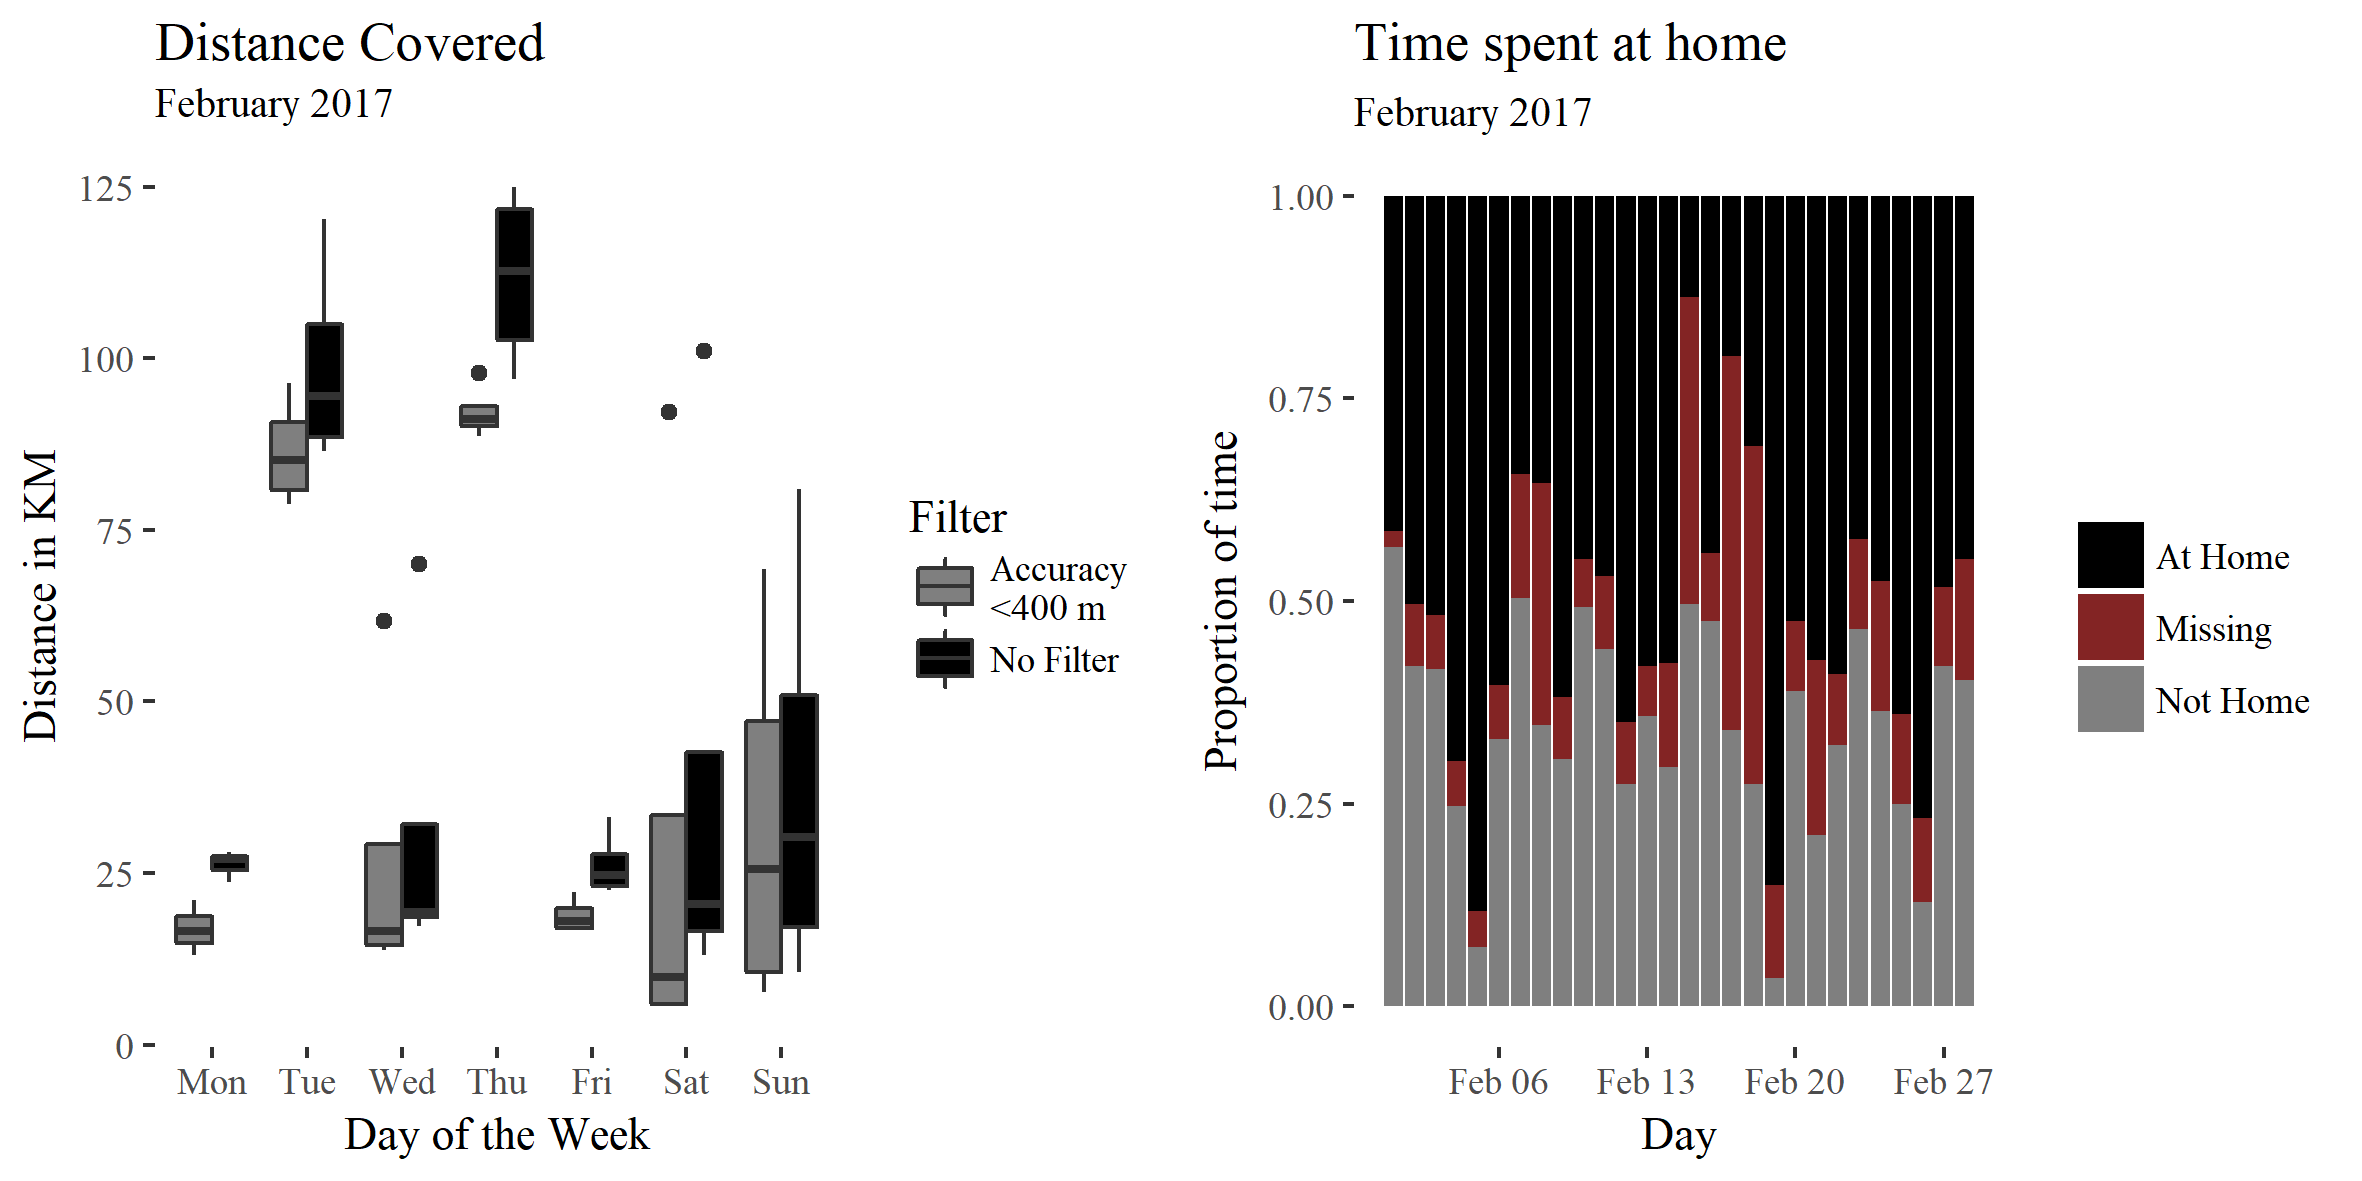
\includegraphics[width=1\linewidth]{img/aggPlot} \caption{Proportion of time spent at home  and distance travelled in February 2017. We estimate time spent at home by calculating the mean lattitude and longitude for every 5 minute time period in the month. The user is coded as at home if within 250 meters of the home coordiantes. One can see that several days have long periods with missing data. More accurate estimates can be reached by imputing the missing measurements. As for distance travelled, it is evident that although the behavioural trends remain the same, the absolute estimate of distance travelled varies depending on the filter.}\label{fig:aggrePlot}
\end{figure}

\subsubsection{Accuracy in location
logs}\label{accuracy-in-location-logs}

Google location history provides a measure of accuracy that is given in
meters such that it represents the radius of a 67\% confidence circle.
In the example data set the distribution of accuracy is highly right
skewed, with a median of 28, \(\mu = 127\) and the maximum value at 26
km. Palmius et al. (2017) note that in their Android based custom logs
inaccurate location values are interspersed between more accurate
location values at higher sample rates per hour. We observe similar
patterns in secondary logs. Figure \ref{fig:accuracyPlot} shows how
accuracy can vary as a function of user behaviour, time and location.
Inaccurate measures are often followed by more accurate measures. Most
notably, low accuracy often (but not always) is associated with movement
(Figure \ref{fig:accuracyPlot2}). Stationary accuracy varies depending
on phone battery level, wifi connection and user phone use. There are
several recurring low-accuracy points, possibly the result of cell-phone
tower triangulation.

\begin{figure}
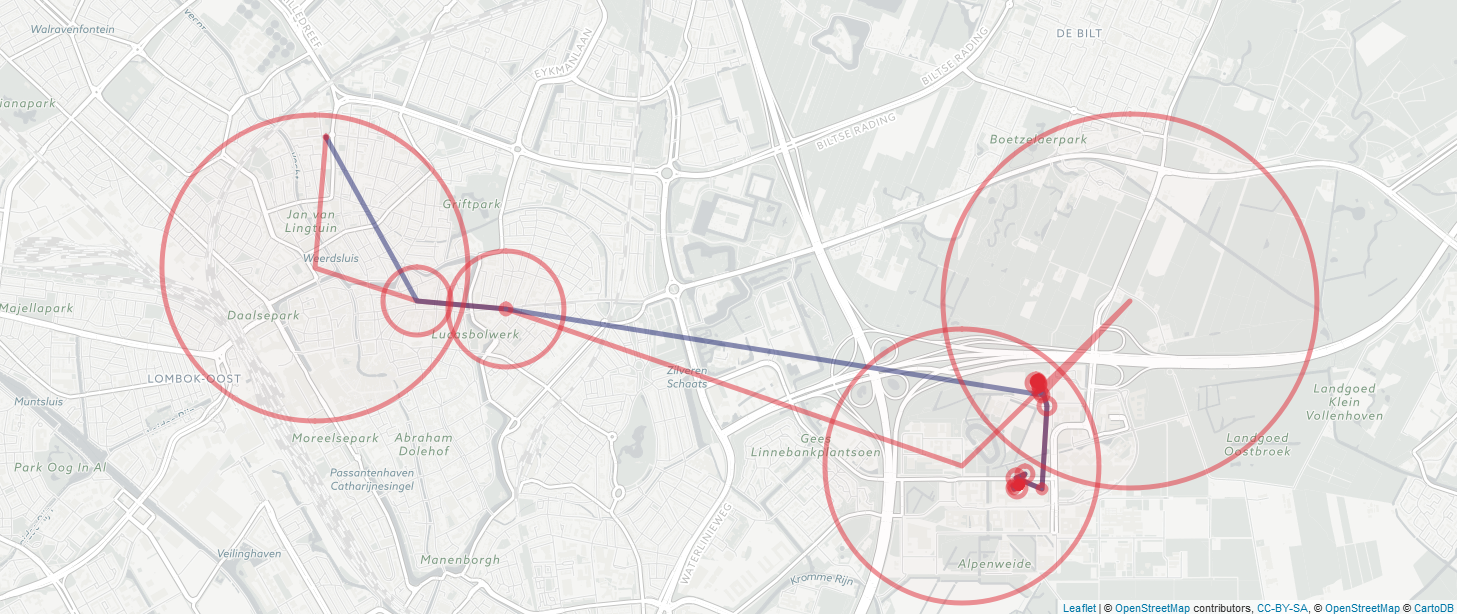
\includegraphics[width=1\linewidth]{img/journeyTillMiddayBoaz} \caption{Measurement accuracy of each logged measurement of a morning journey on February 15th 2017. This includes all measurements from midnight to midday. The red circles denote the accuracy of all logged measurement points (the raw data). The points connected in time are connected by a line. The blue line shows the path without the most inaccurate (accuracy > 400 meters) points filtered out. The red line shows the path with all measurements included. }\label{fig:accuracyPlot}
\end{figure}

\begin{figure}
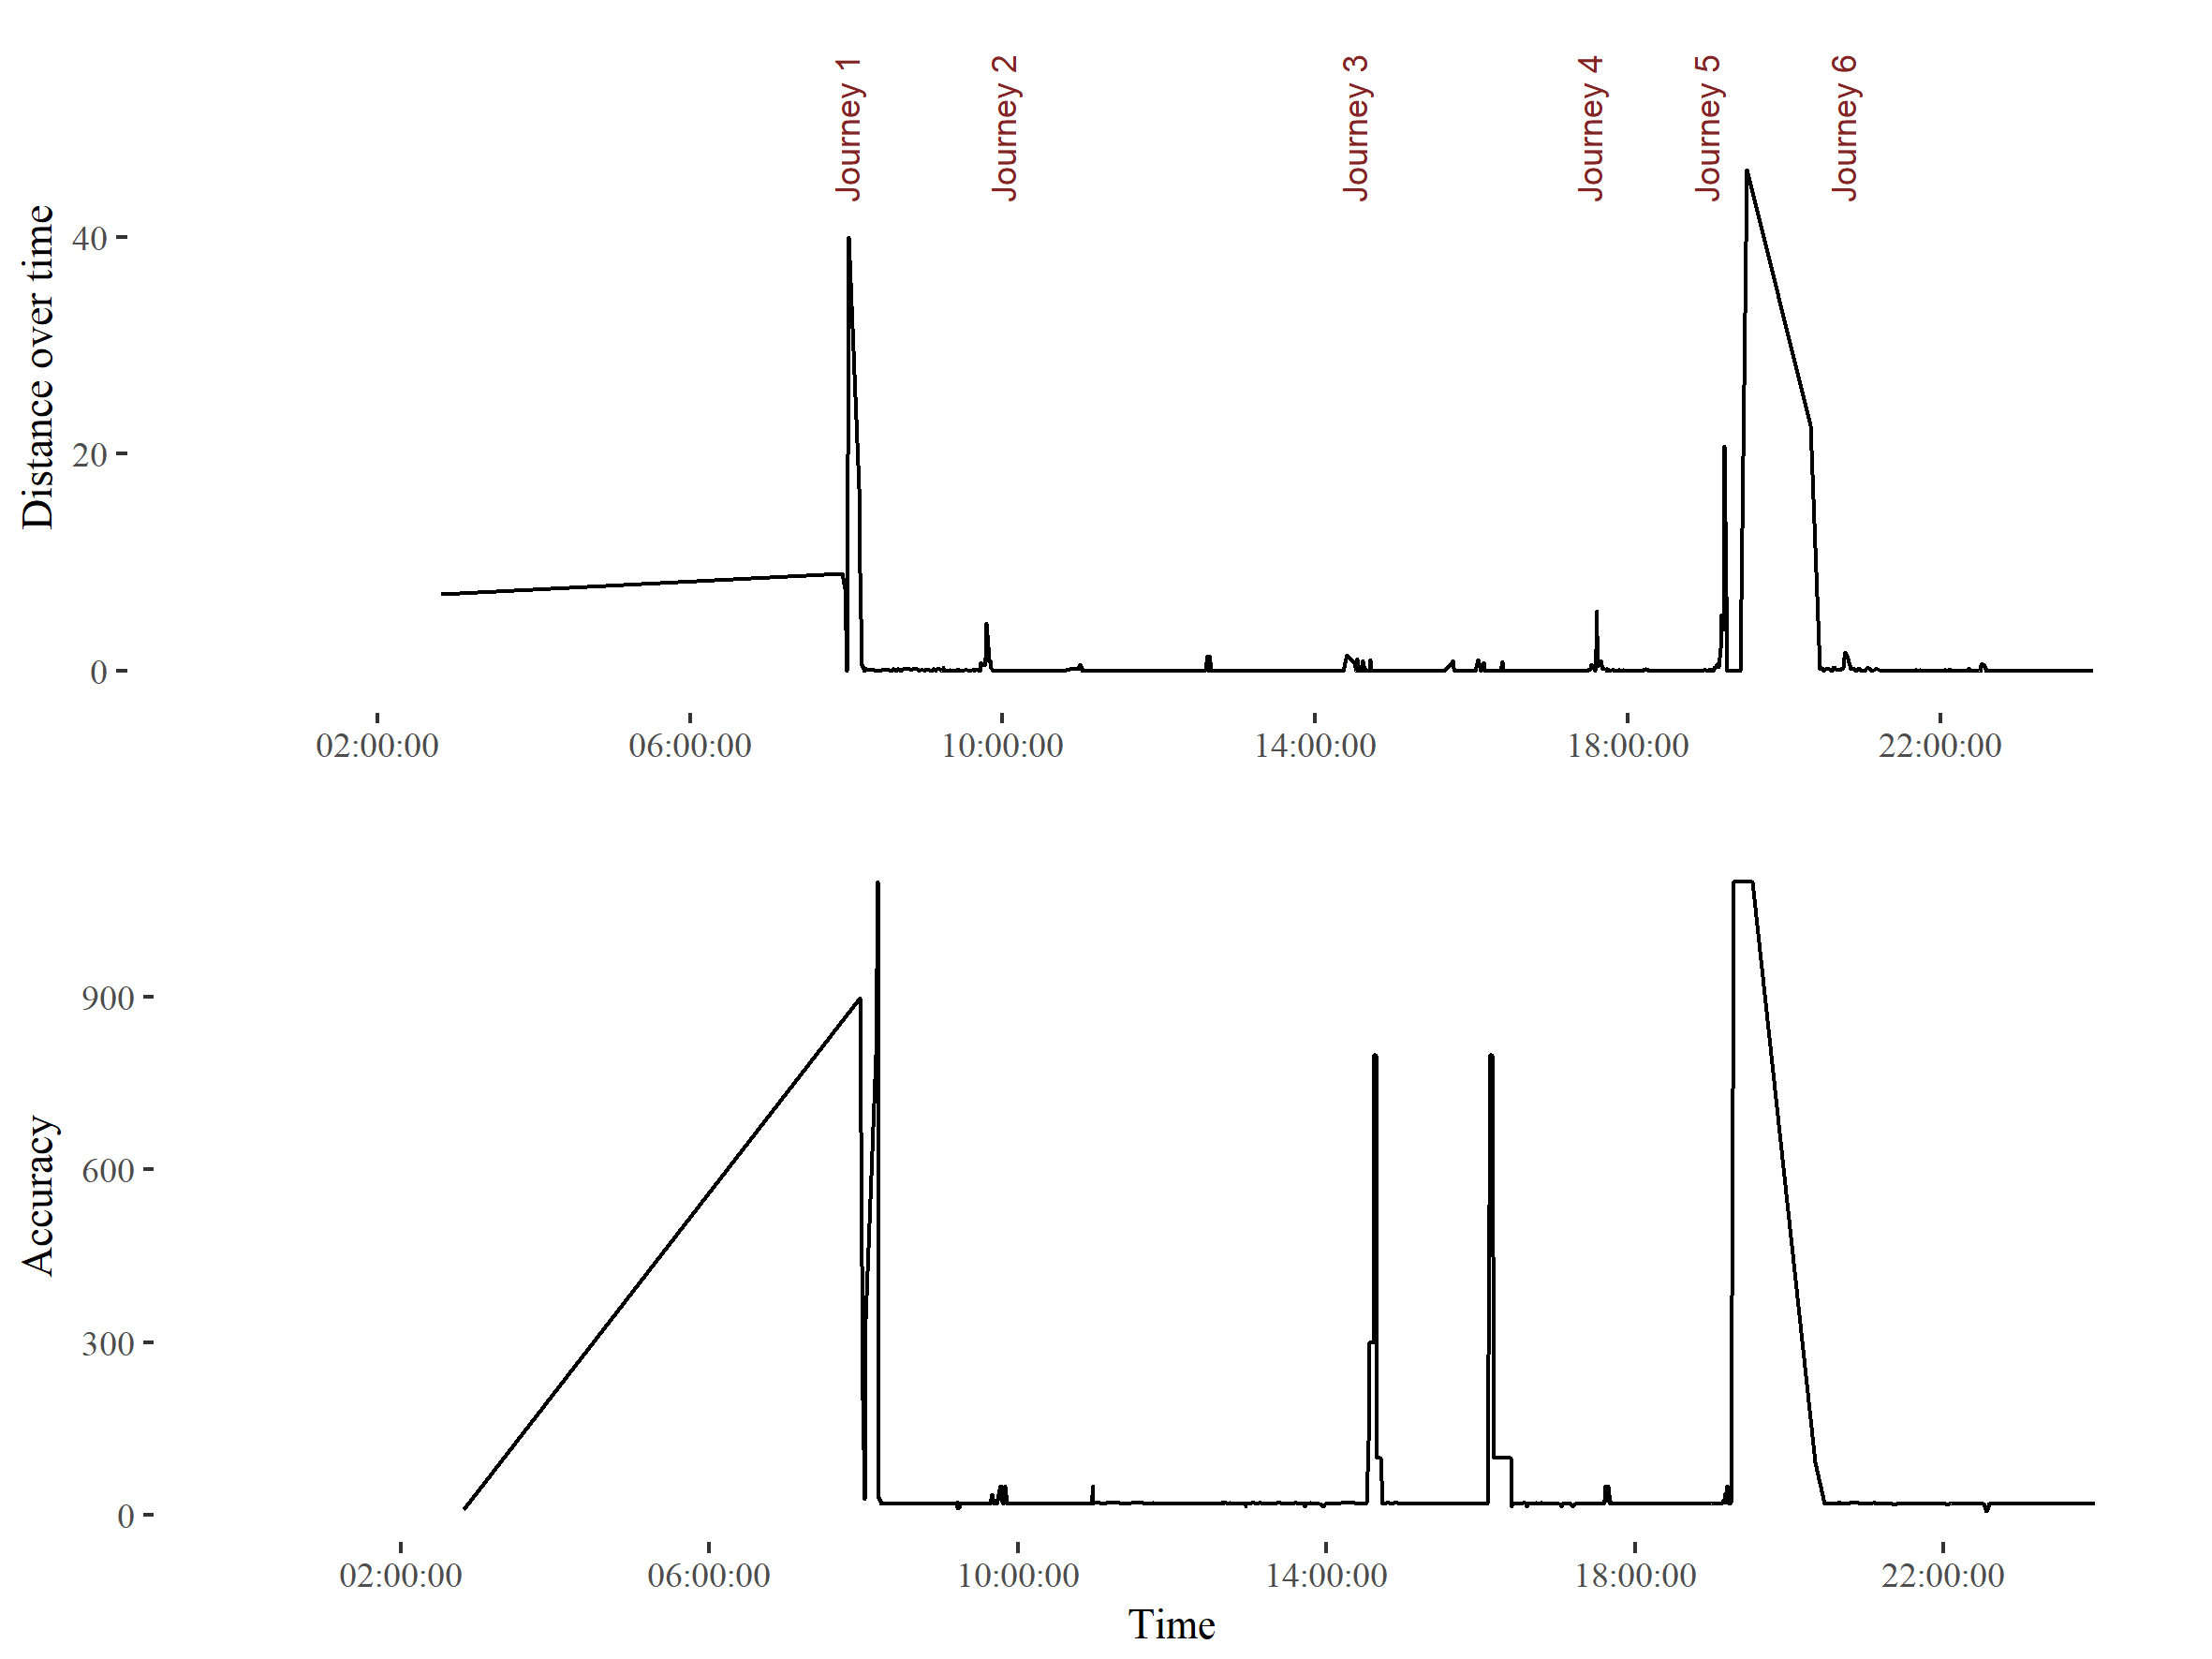
\includegraphics[width=1\linewidth]{img/accuracyLocShift} \caption{Measures of user activity and measurement accuracy on February 15th 2017.The upper chart shows the distance from the next measured point in meters over the course of the day. All journeys are labled at the top of the chart. The first peak corresponds to the first journey from the user's home to a gym around 8am. The second, smaller peak before 10 reflects a journey from the gym to the nearby lecture theatre. Both journeys can be seen in Figure 2. All other journeys are not shown in Figure 2. The large jump between journey 5 and 6 is measurement error. The lower chart shows the accuracy over the course of the day. The figure shows that measurement inaccuracy is sometimes related to the movement of the individual.}\label{fig:accuracyPlot2}
\end{figure}

\subsubsection{Missingness}\label{missingness}

Over 54\% of the data is missing for the entire duration of the log.
This may be misleading as there are several long periods with no
measurements whatsoever (see Figure \ref{fig:longMeasurementsPerDay}).
For days which were not entirely missing, approximately 22\% of all five
minute segments were missing. The structure of missingness of a day with
measurements is shown in Figure \ref{fig:measurementsPerDay}. As you can
see, there are several long periods over the course of the log for which
there are no measurements. Moreover, even during a single day there are
continuous periods where there is missing data, mostly during the late
hours of the night in this case.

\begin{figure}
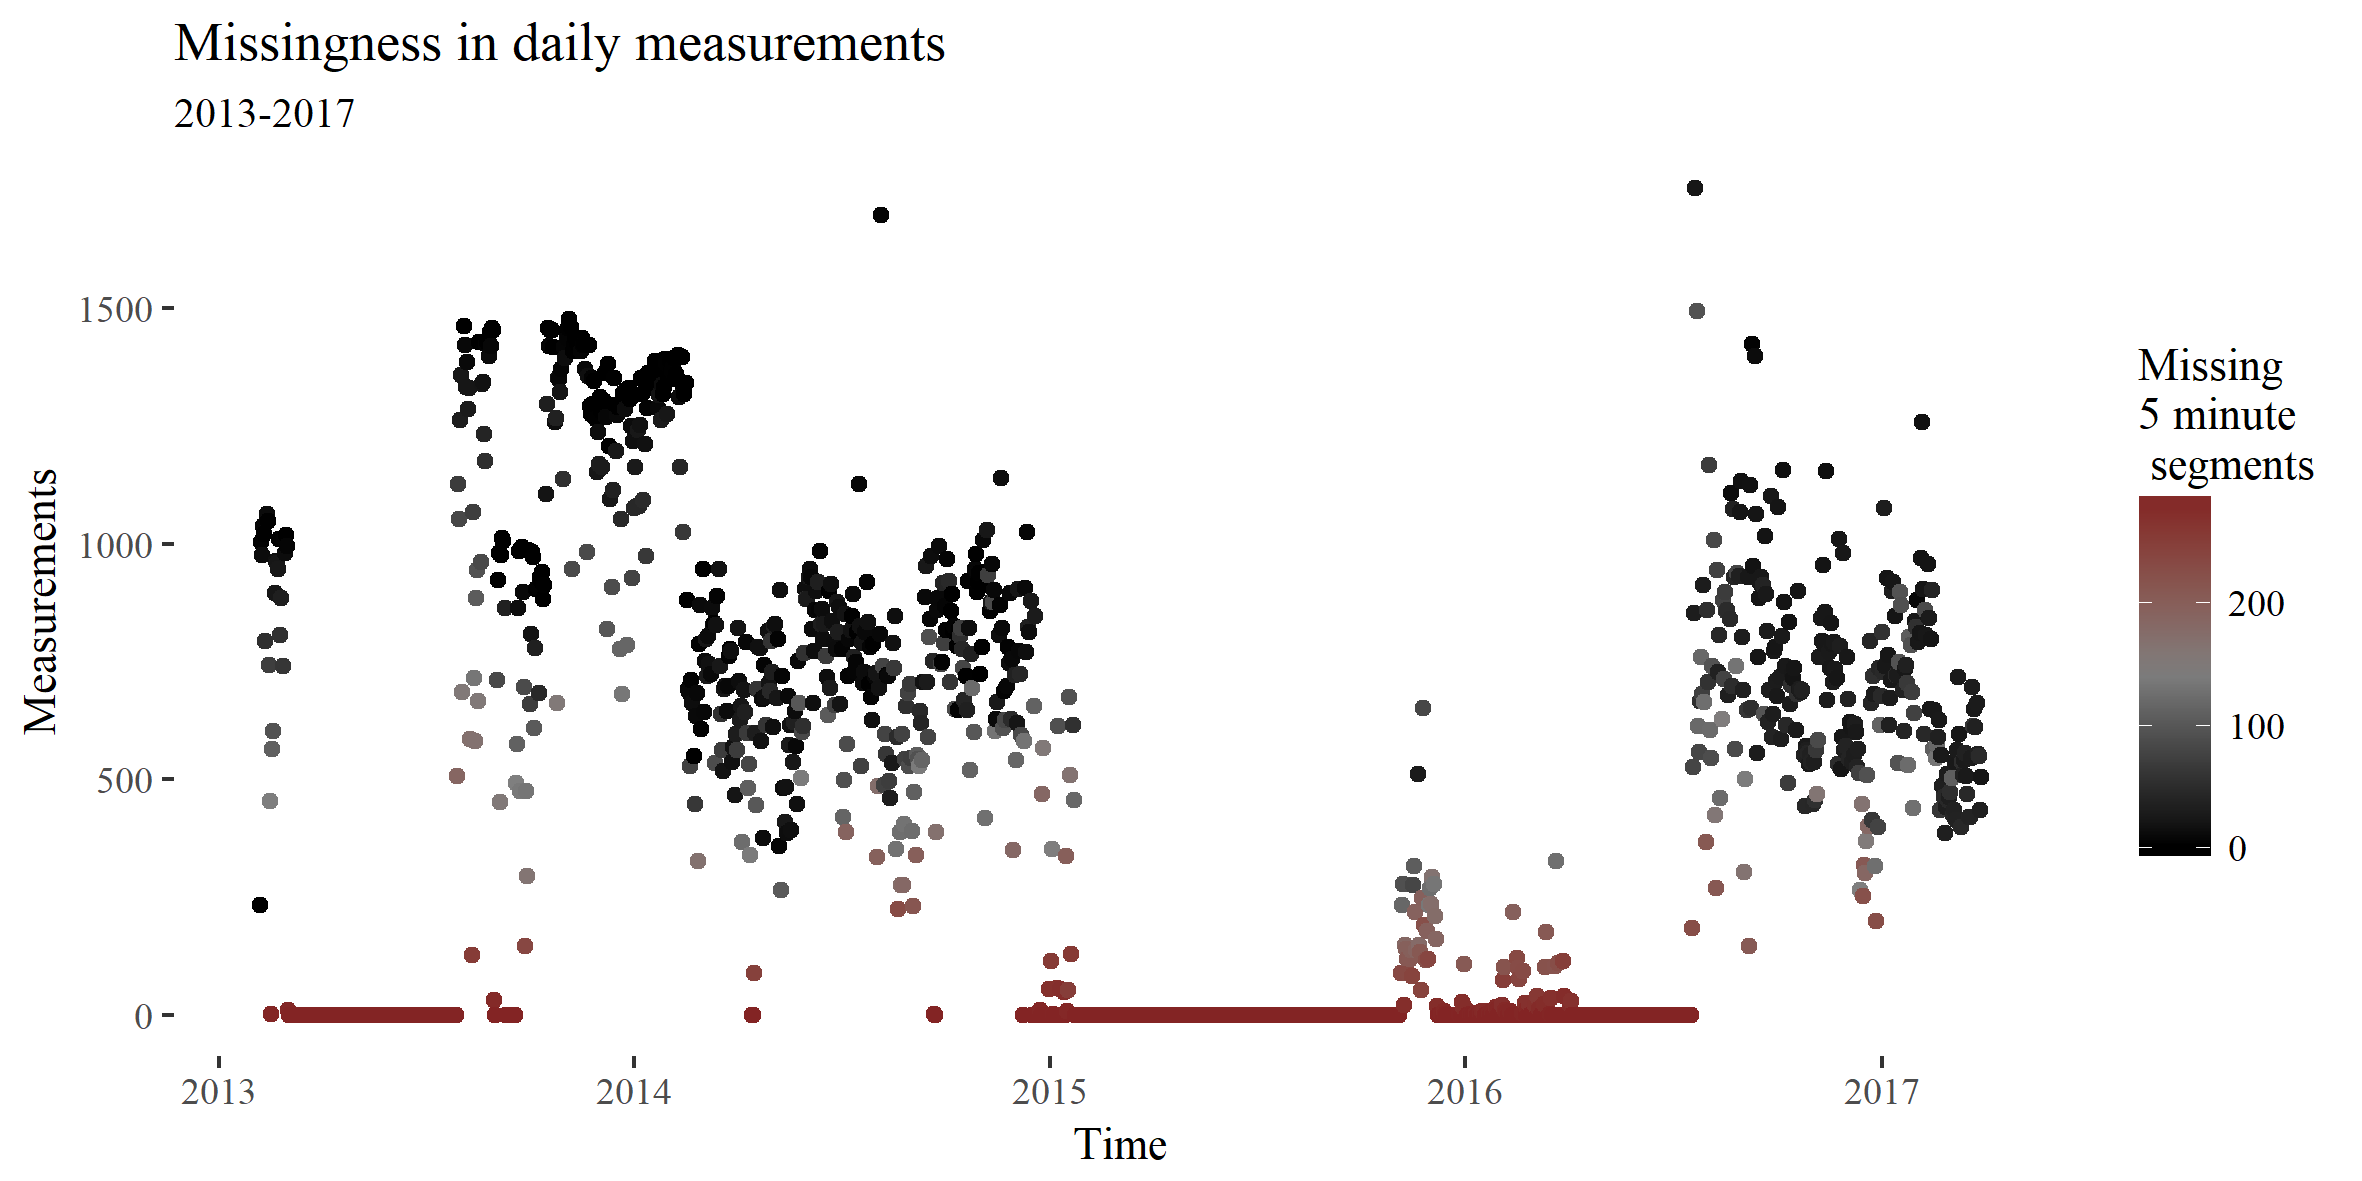
\includegraphics[width=1\linewidth]{img/missingdayBoaz5min} \caption{Example of missing data over the entire duration of the log. The x-axis denotes time, the y-axis shows how many measurements are made and each point is a five minute window. For this day there were several periods with no information. These points are filled with red and lie on the x-axis.}\label{fig:longMeasurementsPerDay}
\end{figure}

\begin{figure}
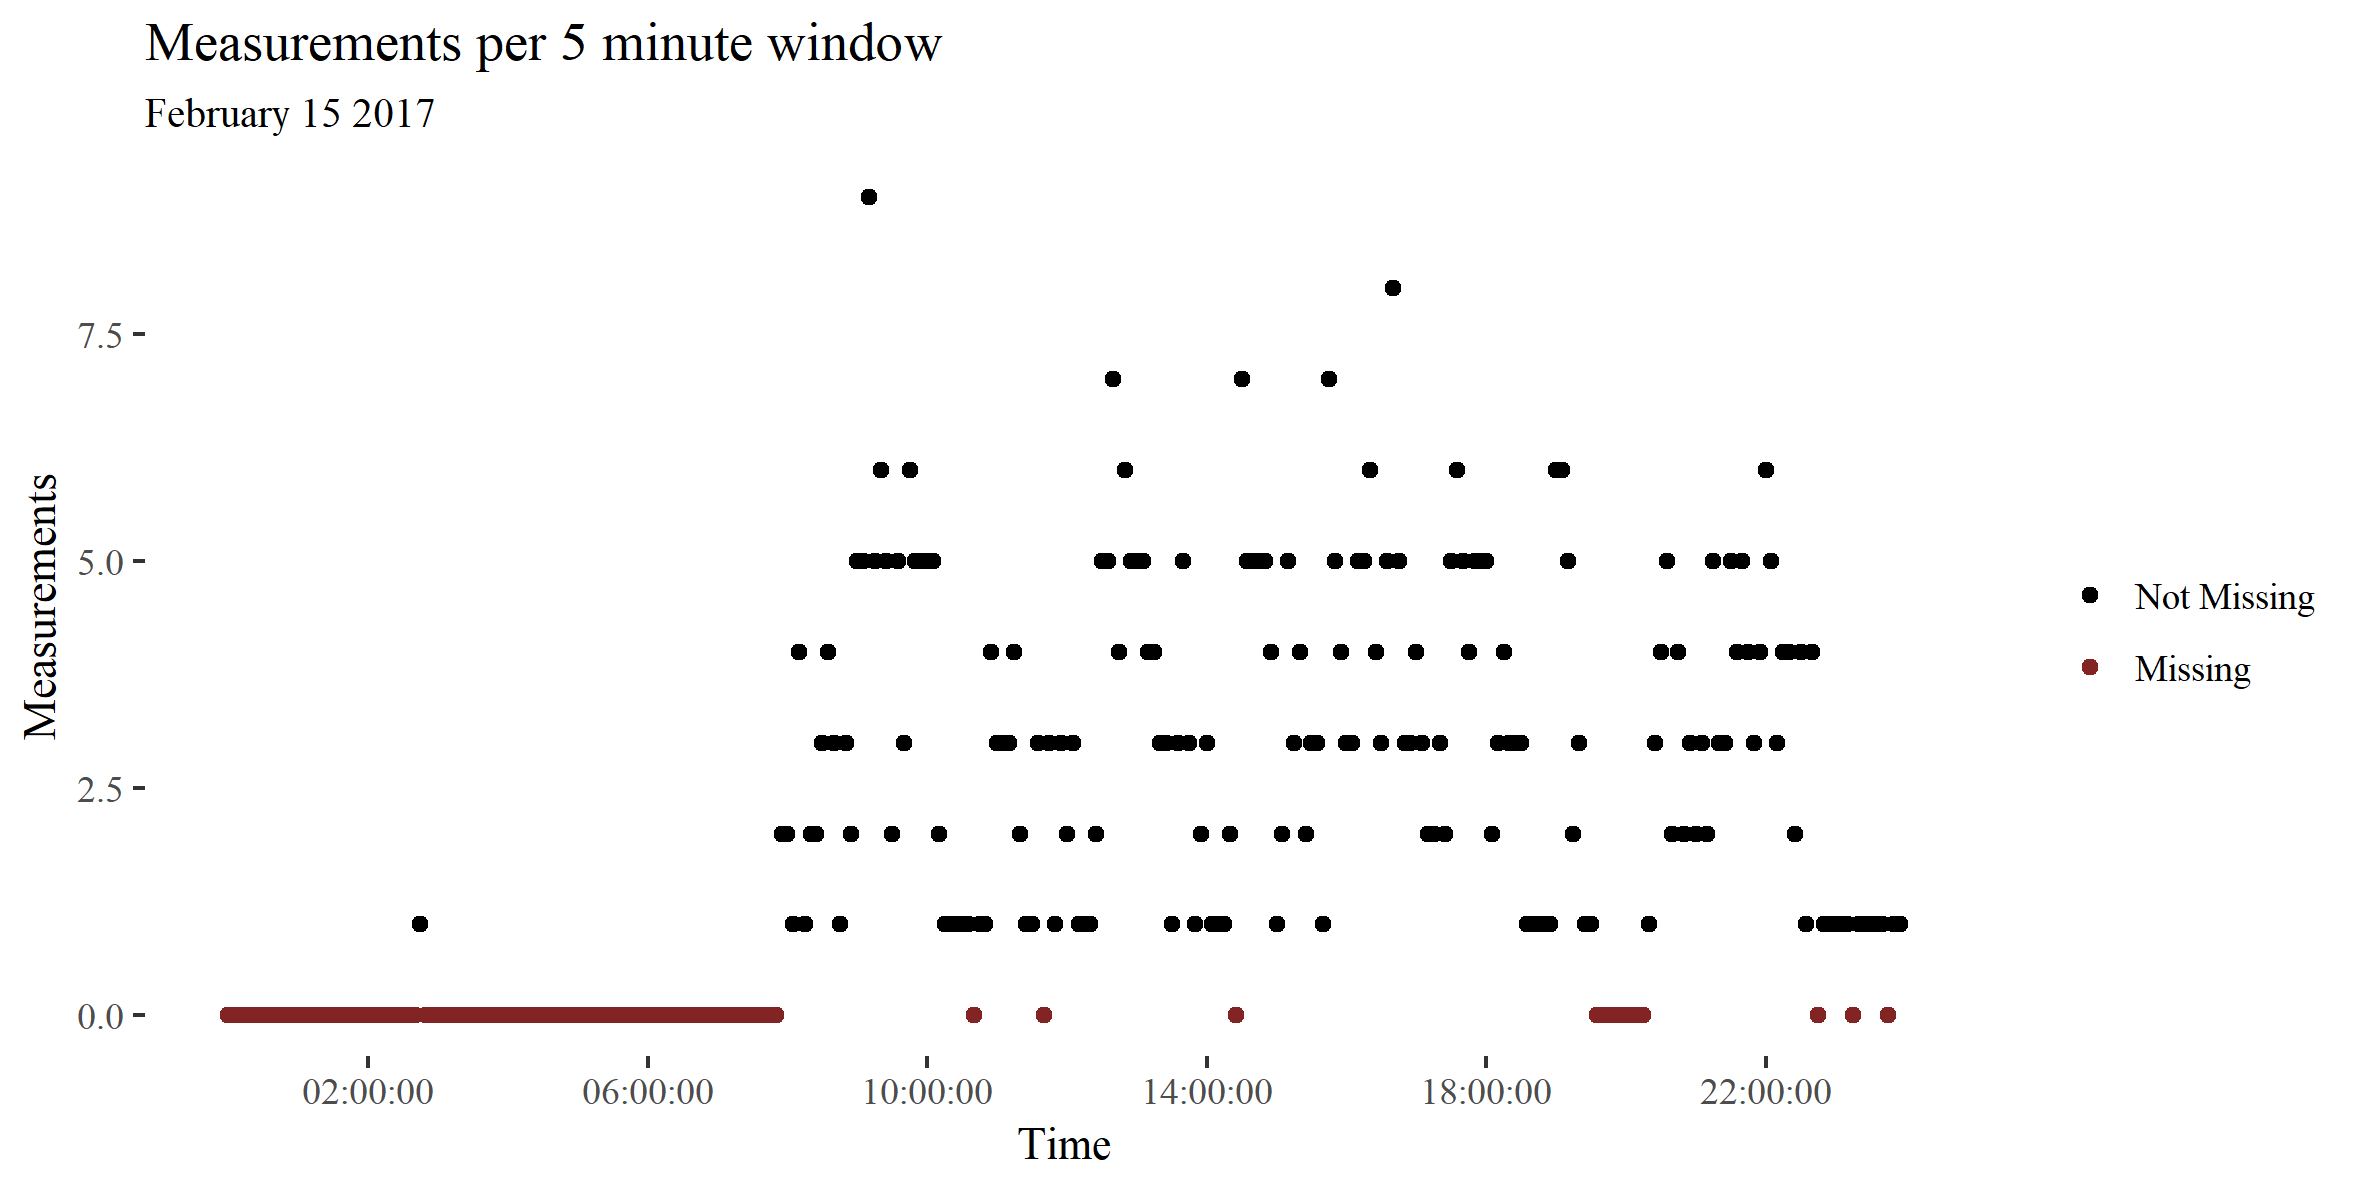
\includegraphics[width=1\linewidth]{img/missingBoaz5minExample} \caption{Example of missing data on February 15th 2017. The x-axis denotes time, the y-axis shows how many measurements are made and each point is a five minute window. For this day there were several periods with no information. These points are filled with red and lie on the x-axis. Missingness over long time periods is related to the type of device the user has.}\label{fig:measurementsPerDay}
\end{figure}

\section{Methods}\label{methods}

\subsection{Two-dimensional projections and
notation}\label{two-dimensional-projections-and-notation}

GPS measurements provide us with coordinates on the surface of the
earth. Because most mobility metrics are computed for data in
\(\mathbb{R}^2\), we are interested in mapping these \(\mathbb{R}^3\)
measurements on a 2D Euclidean plane. Projecting three dimensional
measurements onto a two dimensional plane results in distortion. To
minimise errors we borrow an error minimising projection method from
Barnett and Onnela (2016).

Having thus converted lattitude and longitude onto coordinates unique to
each individual, let a person's true location on this two-dimensional
plane be \(G(t) = [G_x(t) G_y(t)]\) where \(G_x(t)\) and \(G_y(t)\)
denote the location of the individual at time \(t\) on the x-axis and
y-axis respectively. Moreover, let \(D \in \mathbb{R}^2\) be the
recorded data containing lattitude and longitude. In addition, let \(a\)
denote the estimated accuracy of the recorded data. accuracy. \(G(t)\),
\(D\) and \(a\) are indexed by time labled by the countable set
\(t = t_1 < ... < t_{n+1}\). For simplicity, let each entry in the
discrete index set \(t\) represent a 5 minute window. The measure of
accuracy \(a_t\) is given in meters such that it represents the radius
of a 67\% confidence circle. If \(D_t = \emptyset\) it is considered
\emph{missing} and it is not missing otherwise.

When several data sets are available from individuals living in
overlapping areas we can construct a \(t \times i\) matrix \(M\) where
the entry \(M(t,i)\) contains \(G(t)\) for the individual \(i\).

\subsection{Selecting candidate
models}\label{selecting-candidate-models}

There is no golden standard or established practice in how to deal with
missing data in GPS logs. Researchers are generally vague about what
practices they follow (Jankowska et al., 2015). Ostensibly this is
because they are unaware of possible solutions. In an attempt to
elucidate the topic, we explore potential solutions. We will argue that
extensively used spatiotemporal methods, such as state space models
(SSMs), are not well suited to deal with human mobility patterns. We
also discuss in detail two approaches which deal explicitly with
mobility patterns from custom or secondary logs (Barnett \& Onnela,
2016; Palmius et al., 2017 ).

There is a vast literature on using SSMs in spatiotemporal statistics.
For example, ecologists have used SSMs to explain how animals interact
with their environment (Patterson, Thomas, Wilcox, Ovaskainen, \&
Matthiopoulos, 2008). These models can be quite complex. Preisler, Ager,
Johnson, and Kie (2004) uses Markovian movement processes to
characterise the effect of roads, food patches and streams on cyclical
elk movements. The most well studied SSM is the Kalman filter, which is
the optimal algorithm for inferring linear Gaussian systems. The
extended Kalman filter is the de facto standard for GPS navigation (Z.
Chen \& Brown, 2013). The advantage of state space models is that they
are flexible, deal with measurement inaccuracy, include information from
different sources and can be used in real time.

For us, the main limitation of SSMs is that they ignore regular movement
routines. For instance, humans tend to go to work on weekdays and sleep
at night. Because SSMs are based on the Markov property, they cannot
incorporate this information. The estimated location \(G(t)\) at
timepoint \(t\) is often based only upon measurements \(D_t\),
\(D_{t-1}\) and ignores all \(D_{t-i}|i\geq2\). Hierarchical structuring
and conditioning on a larger context have been suggested as ways to add
periodicity to Markovian models. These solutions are often
computationally intractable or unfeasible (Sadilek \& Krumm, 2016). For
this reason we do not consider SSMs to be useful for imputing missing
data. Nonetheless, they could be of use in filtering noise.

In climate or geological research spatiotemporal imputation methods are
often used. For instance, the CUTOFF method estimates missing values
using the nearest observed neighbours (Feng, Nowak, O'Neill, \& Welsh,
2014 ). The authors illustrate their example using rainfall data from
gauging stations across Australia. Similarly, Z. Zhang et al. (2017) use
a variety of machine learning methods to impute missing values. The
example provided relates to underground water data. Generally these
models assume fixed measurement stations (such as rainfall gauging
stations).

For this reason they cannot be easily applied to missing mobility
tracks. Feng et al. (2014) claim their model could be used to establish
mobility patterns. This may be possible by dividing the sample space
into rasters. Each raster would be analogous to a measurement station.
These artificial stations could \enquote{measure} the probability of the
individual being there. To our knowledge such models have not been
implemented for mobility traces and seems computationally inefficient.

On the other hand, a few researchers have explicitly attempted to impute
missing data from human mobility patterns. Palmius et al. (2017) deal
with the measuremement inaccuracy of \(D\) in custom logs by removing
from the data set all unique low-accuracy \(a\) data points that had
\(\frac{d}{dt}D > 100 \frac{km}{h}\). Subsequently the researchers down
sample the data to a sample rate of 12 per hour using a median filter.
Moreover, Palmius et al. (2017) explain:

\begin{quote}
\enquote{If the standard deviation of {[}\(D\){]} in both latitude and
longitude within a 1 h epoch was less than 0.01 km, then all samples
within the hour were set to the mean value of the recorded data,
otherwise a 5 min median filter window was applied to the recorded
latitude and longitude in the epoch}.
\end{quote}

Missing data was imputed using the mean of measurements close in time if
the participant was recorded within 500m of either end of a missing
section and the missing section had a length of \(\leq 2h\) or
\(\leq 12h\) after 9pm.

Barnett and Onnela (2016) follow a different approach which is, to the
best of our knowledge, the only pricipled approach to dealing with
missing data in human mobility data. Barnett and Onnela (2016) work with
custom logs where location is measured for 2 minutes and subsequently
not measured for 10 minutes. In the words of the authors, Barnett and
Onnela (2016) handle missing data by:

\begin{quote}
\enquote{simulat{[}ing{]} flights and pauses over the period of
missingness where the direction, duration, and spatial length of each
flight, the fraction of flights versus the fraction of pauses, and the
duration of pauses are sampled from observed data.}
\end{quote}

This method can be extended to imputing the data based on temporally,
spatially or periodically close flights and pauses. In other words, for
a given missing period, the individual's mobility can be estimated based
on measured movements in that area, at that point in time or movements
in the last 24 hours (\emph{circadian proximity}).

\subsubsection{Datasets \& Analyses}\label{datasets-analyses}

The data used to train the imputation methods was collected between 2013
and 2017 on different Android devices from several individuals (Table
\ref{tab:datadetailsTable}).

\begin{lltable}
\begin{longtable}{llllll}\noalign{\getlongtablewidth\global\LTcapwidth=\longtablewidth}
\caption{\label{tab:datadetailsTable}Table with descriptives about the data sets used to build the imputation methods. Missing data stands for the proportion of missing 5 minute windows within days that were not missing entirely.}\\
\toprule
Log duration & Logged days & Observations & Missing
days & Missing
data & Mean Accuracy\\
\midrule
2013-02-06 to 2017-03-29 & 1,512.00 & 646,376.00 & 635.00 & 0.22 & 127.78\\
2016-07-14 to 2017-05-10 & 300.00 & 158,382.00 & 3.00 & 0.41 & 1,394.60\\
2014-01-22 to 2017-01-23 & 1,097.00 & 814,941.00 & 80.00 & 0.25 & 121.83\\
\bottomrule
\end{longtable}
\end{lltable}

In addition to the secondary logs, participants also volunteered to
carry with them a specialised GPS tracker for a week. This specialised
log was used to evaluate the models.

Analyses were performed using R and a multitude of other statistical
packages (Arnold, 2017; Auguie, 2017; Aust, 2016; Bivand, Pebesma, \&
Gomez-Rubio, 2013; Cheng, Karambelkar, \& Xie, 2017; Francois, 2017; E.
J. Pebesma \& Bivand, 2005; R Core Team, 2017; RStudio Team, 2015;
Thoen, 2017; Vaughan \& Dancho, 2017; Wickham, 2009, 2017; Wickham \&
Henry, 2017; Wickham, Francois, Henry, \& Muller, 2017).

\subsubsection{Data pre-processing \&
filtering}\label{data-pre-processing-filtering}

The goal of filtering was to remove noise from the measurements and to
aggregate multiple measurements into 12 per hour. Three different
filtering methods were tested:

\begin{enumerate}
\def\labelenumi{\arabic{enumi}.}
\tightlist
\item
  The filtered rolling-median downsampling method described by Palmius
  et al. (2017).
\item
  A weighted mean approach taking \(f(a)\) as a weight.
\item
  A Kalman filter commonly used for GPS measurements (Doust, 2013).
\end{enumerate}

The output of all of these methods was taken as the input of the
imputation methods.

\subsubsection{Imputation methods}\label{imputation-methods}

Four imputation methods were selected in order to cover a wide range of
techniques applied in the literature:

\begin{enumerate}
\def\labelenumi{\arabic{enumi}.}
\tightlist
\item
  Mean imputation as described by Palmius et al. (2017).
\item
  The model developed by Barnett and Onnela (2016) using both spatial
  and temporal proximity.
\item
  Simple linear interpolation was used as a benchmark model.
\end{enumerate}

\subsubsection{Evaluation criteria}\label{evaluation-criteria}

The entire length of the secondary logs were used as a training set. The
specialised logs were used as a test set. The missing data imputation
models were evaluated both directly, and on two computed measures:
amount of trips made and distance traveled.

The direct evaluation involved calculating the error of each \(D_t\)
compared to \(G(t)\) approximated by the specialised log. The error
measures used were root mean square error (RMSE) and mean absolute error
(MAE).

The evaluation on computed measures involved calculating a mobility
trace following the rectangular method of Rhee, Shin, Hong, Lee, and
Chong (2007) for each imputed dataset. Like Barnett and Onnela (2016) we
calculate bias by substracting the estimated measure under each approach
for the same measure calculated on the full data. For simulation-based
imputation approaches a mean value over 100 samples was taken.

Each imputation method used each of the three filtering methods as an
input. Thus in the end we end up with eight methods to evaluate, three
for each filtering method as well as four for each imputation method.

\newpage

\section{References}\label{references}

\setlength{\parindent}{-0.5in} \setlength{\leftskip}{0.5in}

\hypertarget{refs}{}
\hypertarget{ref-ggthemes}{}
Arnold, J. B. (2017). \emph{Ggthemes: Extra themes, scales and geoms for
'ggplot2'}. Retrieved from
\url{https://CRAN.R-project.org/package=ggthemes}

\hypertarget{ref-gridExtra}{}
Auguie, B. (2017). \emph{GridExtra: Miscellaneous functions for ``grid''
graphics}. Retrieved from
\url{https://CRAN.R-project.org/package=gridExtra}

\hypertarget{ref-citr}{}
Aust, F. (2016). \emph{Citr: 'RStudio' add-in to insert markdown
citations}. Retrieved from \url{https://CRAN.R-project.org/package=citr}

\hypertarget{ref-barnett_inferring_2016}{}
Barnett, I., \& Onnela, J.-P. (2016). Inferring Mobility Measures from
GPS Traces with Missing Data. \emph{arXiv:1606.06328 {[}Stat{]}}.
Retrieved from \url{http://arxiv.org/abs/1606.06328}

\hypertarget{ref-sp2}{}
Bivand, R. S., Pebesma, E., \& Gomez-Rubio, V. (2013). \emph{Applied
spatial data analysis with R, second edition}. Springer, NY. Retrieved
from \url{http://www.asdar-book.org/}

\hypertarget{ref-chen_practical_2006}{}
Chen, M. Y., Sohn, T., Chmelev, D., Haehnel, D., Hightower, J., Hughes,
J., \ldots{} Varshavsky, A. (2006). Practical Metropolitan-Scale
Positioning for GSM Phones. In \emph{UbiComp 2006: Ubiquitous Computing}
(pp. 225--242). Springer, Berlin, Heidelberg.
doi:\href{https://doi.org/10.1007/11853565_14}{10.1007/11853565\_14}

\hypertarget{ref-chen_state_2013}{}
Chen, Z., \& Brown, E. N. (2013). State space model.
\emph{Scholarpedia}, \emph{8}(3), 30868.
doi:\href{https://doi.org/10.4249/scholarpedia.30868}{10.4249/scholarpedia.30868}

\hypertarget{ref-leaflet}{}
Cheng, J., Karambelkar, B., \& Xie, Y. (2017). \emph{Leaflet: Create
interactive web maps with the javascript 'leaflet' library}. Retrieved
from \url{https://CRAN.R-project.org/package=leaflet}

\hypertarget{ref-commission_protecting_2017}{}
Commission, E. (2017). Protecting your data: Your rights - European
Commission. Retrieved from
\url{http://ec.europa.eu/justice/data-protection/individuals/rights/index_en.htm}

\hypertarget{ref-delclos-alio_keeping_2017}{}
Delclòs-Alió, X., Marquet, O., \& Miralles-Guasch, C. (2017). Keeping
track of time: A Smartphone-based analysis of travel time perception in
a suburban environment. \emph{Travel Behaviour and Society},
\emph{9}(Supplement C), 1--9.
doi:\href{https://doi.org/10.1016/j.tbs.2017.07.001}{10.1016/j.tbs.2017.07.001}

\hypertarget{ref-doust_smoothing_2013}{}
Doust, P. (2013). \emph{Smoothing - Smooth GPS data - Stack Overflow}.
Retrieved from
\url{https://stackoverflow.com/questions/1134579/smooth-gps-data}

\hypertarget{ref-duncan_portable_2013}{}
Duncan, S., Stewart, T. I., Oliver, M., Mavoa, S., MacRae, D., Badland,
H. M., \& Duncan, M. J. (2013). Portable global positioning system
receivers: Static validity and environmental conditions. \emph{American
Journal of Preventive Medicine}, \emph{44}(2), e19--29.
doi:\href{https://doi.org/10.1016/j.amepre.2012.10.013}{10.1016/j.amepre.2012.10.013}

\hypertarget{ref-feng_cutoff:_2014}{}
Feng, L., Nowak, G., O'Neill, T., \& Welsh, A. (2014). CUTOFF: A
spatio-temporal imputation method. \emph{Journal of Hydrology},
\emph{519}, 3591--3605.
doi:\href{https://doi.org/10.1016/j.jhydrol.2014.11.012}{10.1016/j.jhydrol.2014.11.012}

\hypertarget{ref-bibtex}{}
Francois, R. (2017). \emph{Bibtex: Bibtex parser}. Retrieved from
\url{https://CRAN.R-project.org/package=bibtex}

\hypertarget{ref-goodchild_toward_2010}{}
Goodchild, M. F., \& Janelle, D. G. (2010). Toward critical spatial
thinking in the social sciences and humanities. \emph{GeoJournal},
\emph{75}(1), 3--13.
doi:\href{https://doi.org/10.1007/s10708-010-9340-3}{10.1007/s10708-010-9340-3}

\hypertarget{ref-grunerbl_smartphone-based_2015}{}
Grünerbl, A., Muaremi, A., Osmani, V., Bahle, G., Ohler, S., Tröster,
G., \ldots{} Lukowicz, P. (2015). Smartphone-based recognition of states
and state changes in bipolar disorder patients. \emph{IEEE Journal of
Biomedical and Health Informatics}, \emph{19}(1), 140--148.
doi:\href{https://doi.org/10.1109/JBHI.2014.2343154}{10.1109/JBHI.2014.2343154}

\hypertarget{ref-harari_using_2016}{}
Harari, G. M., Lane, N. D., Wang, R., Crosier, B. S., Campbell, A. T.,
\& Gosling, S. D. (2016). Using Smartphones to Collect Behavioral Data
in Psychological Science: Opportunities, Practical Considerations, and
Challenges. \emph{Perspectives on Psychological Science}, \emph{11}(6),
838--854.
doi:\href{https://doi.org/10.1177/1745691616650285}{10.1177/1745691616650285}

\hypertarget{ref-jankowska_framework_2015}{}
Jankowska, M. M., Schipperijn, J., \& Kerr, J. (2015). A Framework For
Using GPS Data In Physical Activity And Sedentary Behavior Studies.
\emph{Exercise and Sport Sciences Reviews}, \emph{43}(1), 48--56.
doi:\href{https://doi.org/10.1249/JES.0000000000000035}{10.1249/JES.0000000000000035}

\hypertarget{ref-lamarca_place_2005}{}
LaMarca, A., Chawathe, Y., Consolvo, S., Hightower, J., Smith, I.,
Scott, J., \ldots{} Schilit, B. (2005). Place Lab: Device Positioning
Using Radio Beacons in the Wild. In \emph{Pervasive Computing} (pp.
116--133). Springer, Berlin, Heidelberg.
doi:\href{https://doi.org/10.1007/11428572_8}{10.1007/11428572\_8}

\hypertarget{ref-location_history_timeline_2017}{}
Location History, G. (2017). Timeline. Retrieved from
\url{https://www.google.com/maps/timeline?pb}

\hypertarget{ref-palmius_detecting_2017}{}
Palmius, N., Tsanas, A., Saunders, K. E. A., Bilderbeck, A. C., Geddes,
J. R., Goodwin, G. M., \& Vos, M. D. (2017). Detecting Bipolar
Depression From Geographic Location Data. \emph{IEEE Transactions on
Biomedical Engineering}, \emph{64}(8), 1761--1771.
doi:\href{https://doi.org/10.1109/TBME.2016.2611862}{10.1109/TBME.2016.2611862}

\hypertarget{ref-patterson_statespace_2008}{}
Patterson, T. A., Thomas, L., Wilcox, C., Ovaskainen, O., \&
Matthiopoulos, J. (2008). State--space models of individual animal
movement. \emph{Trends in Ecology \& Evolution}, \emph{23}(2), 87--94.
doi:\href{https://doi.org/10.1016/j.tree.2007.10.009}{10.1016/j.tree.2007.10.009}

\hypertarget{ref-sp1}{}
Pebesma, E. J., \& Bivand, R. S. (2005). Classes and methods for spatial
data in R. \emph{R News}, \emph{5}(2), 9--13. Retrieved from
\url{https://CRAN.R-project.org/doc/Rnews/}

\hypertarget{ref-preisler_modeling_2004}{}
Preisler, H. K., Ager, A. A., Johnson, B. K., \& Kie, J. G. (2004).
Modeling animal movements using stochastic differential equations.
\emph{Environmetrics 15: P. 643-657}. Retrieved from
\url{https://www.fs.usda.gov/treesearch/pubs/33038}

\hypertarget{ref-base}{}
R Core Team. (2017). \emph{R: A language and environment for statistical
computing}. Vienna, Austria: R Foundation for Statistical Computing.
Retrieved from \url{https://www.R-project.org/}

\hypertarget{ref-rhee_human_2007}{}
Rhee, I., Shin, M., Hong, S., Lee, K., \& Chong, S. (2007). Human
Mobility Patterns and Their Impact on Routing in Human-Driven Mobile
Networks. \emph{ACM HotNets 2007}. Retrieved from
\url{http://koasas.kaist.ac.kr/handle/10203/160927}

\hypertarget{ref-rstudio}{}
RStudio Team. (2015). \emph{RStudio: Integrated development environment
for r}. Boston, MA: RStudio, Inc. Retrieved from
\url{http://www.rstudio.com/}

\hypertarget{ref-sadilek_far_2016}{}
Sadilek, A., \& Krumm, J. (2016). Far Out: Predicting Long-Term Human
Mobility. \emph{Microsoft Research}. Retrieved from
\url{https://www.microsoft.com/en-us/research/publication/far-predicting-long-term-human-mobility/}

\hypertarget{ref-saeb_mobile_2015}{}
Saeb, S., Zhang, M., Karr, C. J., Schueller, S. M., Corden, M. E.,
Kording, K. P., \& Mohr, D. C. (2015). Mobile Phone Sensor Correlates of
Depressive Symptom Severity in Daily-Life Behavior: An Exploratory
Study. \emph{Journal of Medical Internet Research}, \emph{17}(7), e175.
doi:\href{https://doi.org/10.2196/jmir.4273}{10.2196/jmir.4273}

\hypertarget{ref-schipperijn_dynamic_2014}{}
Schipperijn, J., Kerr, J., Duncan, S., Madsen, T., Klinker, C. D., \&
Troelsen, J. (2014). Dynamic Accuracy of GPS Receivers for Use in Health
Research: A Novel Method to Assess GPS Accuracy in Real-World Settings.
\emph{Frontiers in Public Health}, \emph{2}, 21.
doi:\href{https://doi.org/10.3389/fpubh.2014.00021}{10.3389/fpubh.2014.00021}

\hypertarget{ref-padr}{}
Thoen, E. (2017). \emph{Padr: Quickly get datetime data ready for
analysis}. Retrieved from \url{https://CRAN.R-project.org/package=padr}

\hypertarget{ref-tibbletime}{}
Vaughan, D., \& Dancho, M. (2017). \emph{Tibbletime: Time aware
tibbles}. Retrieved from
\url{https://CRAN.R-project.org/package=tibbletime}

\hypertarget{ref-wang_smartgpa:_2015}{}
Wang, R., Harari, G., Hao, P., Zhou, X., \& Campbell, A. T. (2015).
SmartGPA: How Smartphones Can Assess and Predict Academic Performance of
College Students. In \emph{Proceedings of the 2015 ACM International
Joint Conference on Pervasive and Ubiquitous Computing} (pp. 295--306).
New York, NY, USA: ACM.
doi:\href{https://doi.org/10.1145/2750858.2804251}{10.1145/2750858.2804251}

\hypertarget{ref-ggplot2}{}
Wickham, H. (2009). \emph{Ggplot2: Elegant graphics for data analysis}.
Springer-Verlag New York. Retrieved from \url{http://ggplot2.org}

\hypertarget{ref-scales}{}
Wickham, H. (2017). \emph{Scales: Scale functions for visualization}.
Retrieved from \url{https://CRAN.R-project.org/package=scales}

\hypertarget{ref-tidyr}{}
Wickham, H., \& Henry, L. (2017). \emph{Tidyr: Easily tidy data with
'spread()' and 'gather()' functions}. Retrieved from
\url{https://CRAN.R-project.org/package=tidyr}

\hypertarget{ref-dplyr}{}
Wickham, H., Francois, R., Henry, L., \& Muller, K. (2017). \emph{Dplyr:
A grammar of data manipulation}. Retrieved from
\url{https://CRAN.R-project.org/package=dplyr}

\hypertarget{ref-wolf_impact_2003}{}
Wolf, J., Oliveira, M., \& Thompson, M. (2003). Impact of Underreporting
on Mileage and Travel Time Estimates: Results from Global Positioning
System-Enhanced Household Travel Survey. \emph{Transportation Research
Record: Journal of the Transportation Research Board}, \emph{1854},
189--198. doi:\href{https://doi.org/10.3141/1854-21}{10.3141/1854-21}

\hypertarget{ref-zenk_how_2009}{}
Zenk, S. N., Schulz, A. J., \& Odoms-Young, A. (2009). How Neighborhood
Environments Contribute to Obesity. \emph{The American Journal of
Nursing}, \emph{109}(7), 61--64.
doi:\href{https://doi.org/10.1097/01.NAJ.0000357175.86507.c8}{10.1097/01.NAJ.0000357175.86507.c8}

\hypertarget{ref-zhang_application_2017}{}
Zhang, Z., Yang, X., Li, H., Li, W., Yan, H., \& Shi, F. (2017).
Application of a novel hybrid method for spatiotemporal data imputation:
A case study of the Minqin County groundwater level. \emph{Journal of
Hydrology}, \emph{553}(Supplement C), 384--397.
doi:\href{https://doi.org/10.1016/j.jhydrol.2017.07.053}{10.1016/j.jhydrol.2017.07.053}






\end{document}
